% !TeX root = ./00.main.tex
\chapter{Trabalhos Relacionados}\label{cha:related}

% % discussão de 2020-02-01
% Aqueles que contenham:
%     - detecção de anomalia em streams
%     - detecção de intrusão em rede com processamento de streams
%     - BigFlow
% %/discussão

% cap 3: Trabalhos relacionados
%     - Artigos sobre o Minas
%     - outros que paralelizaram algoritmos de mineração de 
%        dados/streams alguns online (5-10 refs)
%     - implementação paralelas/distribuídas em dispositivos pequenos
% % 

\begin{resumocap}

Este Capítulo trata dos trabalhos relacionados e estabelece o estado da arte
dos tópicos Detecção de Novidades em Fluxos de Dados, e
Processamento Distribuído de Fluxos de Dados.

\end{resumocap}

% \section{Algoritmo MINAS e Algoritmos Derivados}

\section{Algoritmos de Detecção de Novidades}\label{sec:alg-nd}

\newcommand{\fog}{\emph{fog computing}\xspace}
\newcommand{\cloud}{\emph{cloud computing}\xspace}

\newcommand{\cluster}{\emph{cluster}\xspace}
\newcommand{\clusters}{\emph{clusters}\xspace}

\newcommand{\dataset}{\emph{data set}\xspace}
\newcommand{\datasets}{\emph{data sets}\xspace}
% \clusters é um conjunto de \cluster feito de um \dataset.

O algoritmo MINAS, como já foi discutido na Seção \ref{sec:minas-og}, classifica
exemplos e detecta
novidades em DS e considera em sua composição \emph{concept drift} e
\emph{concept evolution}, sendo capaz de classificar como extensão de classe
conhecida e reconhecer novas classes sem intervenção de especialista
\cite{Faria2016minas}. Neste trabalho, consideram-se algoritmos derivados
aqueles apresentados em trabalhos publicados após 2016 que estendem a
implementação original do MINAS seguindo sua estrutura básica.

\subsection{Algoritmo FuzzyND}

% FuzzyND
% $(n, \mathit{M}, \overline{CF1^x}, SSD^e, t, l)$
% $(n, LS, SS, t, l)$
% A nova estrutura contrapõem a estrutura original
% substituindo a soma linear dos elementos ($LS$) por  e $SS$ por $M$ e $$

O algoritmo FuzzyND, derivado do MINAS é proposto por \citeonline{DaSilva2018}.
FuzzyND incrementa o algoritmo original aplicando a ele teorias de
conjuntos \emph{fuzzy} pela modificação da representação dos \clusters.
A modificação afeta os métodos de construção de \clusters, classificação
de exemplos e detecção de novidades de acordo com a nova representação.

\acronym{F1M}{\emph{Macro F-Score}, acurácia }

A avaliação do algoritmo FuzzyND é feita por meio de experimentos usando 3 
\datasets sintéticos (\emph{MOA3}, \emph{RBF}, \emph{SynEDC})
e comparação com o MINAS.
O método de avaliação utilizado baseia-se na matriz de confusão incremental
descrita por \citeonline{Faria2016nd} extraindo dessa matriz duas métricas:
acurácia (\emph{Macro F-Score}) \cite{Sokolova2009} e
taxa de desconhecidos (\emph{UnkR}) \cite{Faria2016minas}.
Em geral, o algoritmo FuzzyND detecta melhor novidades e, consequentemente,
é mais robusto a valores atípicos (\emph{outlier}), porém perde a capacidade
de reconhecer padrões recorrentes.


% Experiments were evaluated using the incremental confusion-matrix proposed by [27],
% recently been proposed [5]–[9]
% [5] T. Al-Khateeb, M. M. Masud, L. Khan, C. Aggarwal, J. Han, and B.
% Thuraisingham, “Stream classification with recurring and novel class detection
% using class-based ensemble,” in Data Mining (ICDM), 2012 IEEE 12th International
% Conference on. IEEE, 2012, pp. 31–40.
% [6] E. R. de Faria, A. C. P. de Leon Ferreira, J. Gama et al., “Minas:
% multiclass learning algorithm for novelty detection in data streams,” Data
% Mining and Knowledge Discovery, vol. 30, no. 3, pp. 640–680, 2016.
% [7] M. Masud, J. Gao, L. Khan, J. Han, and B. M. Thuraisingham, “Classification
% and novel class detection in concept-drifting data streams under time
% constraints,” IEEE Transactions on Knowledge and Data Engineering, vol. 23, no.
% 6, pp. 859–874, 2011.
% [8] M. M. Masud, Q. Chen, L. Khan, C. Aggarwal, J. Gao, J. Han, and B.
% Thuraisingham, “Addressing concept-evolution in concept-drifting data streams,”
% in Data Mining (ICDM), 2010 IEEE 10th International Conference on. IEEE, 2010,
% pp. 929–934.
% [9] Z. S. Abdallah, M. M. Gaber, B. Srinivasan, and S. Krishnaswamy, “Anynovel:
% detection of novel concepts in evolving data streams,” Evolving Systems, vol. 7,
% no. 2, pp. 73–93, 2016.
% [27] E. R. de Faria, I. R. Goncalves, J. Gama, A. C. P. de Leon Ferreira et al.,
% “Evaluation of multiclass novelty detection algorithms for data streams,” IEEE
% Transactions on Knowledge and Data Engineering, vol. 27, no. 11, pp. 2961–2973,
% 2015.
% [28] M. Sokolova and G. Lapalme, “A systematic analysis of performance measures
% for classification tasks,” Information Processing & Manage- ment, vol. 45, no.
% 4, pp. 427–437, 2009.

\subsection{Algoritmos MINAS-LC e MINAS-BR}\label{sub:minas-derivados}

O algoritmo MINAS-LC é proposto por \citeonline{Costa2019thesis} e trata a classificação
multi-rótulo, porém não trata evoluções de conceito (\emph{Concept Evolution}).
As alterações fundamentais propostas são:
a representação de \cluster onde MINAS-LC troca a etiqueta, que era única, por uma multi-rótulo;
a transformação de problema aplicada ao conjunto de treinamento para transformá-lo de um
conjunto multi-rótulo para um conjunto multi-classe (simplificação)
em duas variações \emph{Label Powerset} e \emph{Pruned Sets} com
mineração de conjunto de itens frequentes.

% Este capítulo apresentou o método MultI-label learNing Algorithm for data
% Streams with Label Combination-based methods (MINAS-LC) e o MultI-label learNing
% Algorithm for data Streams with Binary Relevance transformation (MINAS-BR) para
% CMFCD com latência extrema de rótulos. O MINAS-LC lida com problemas apenas com
% mudanças de conceito. O seu modelo de decisão e composto por microgrupos
% multirrotulados sendo capaz de classificar exemplos em várias classes
% simultaneamente e evoluir ao longo do fluxo de dados. Foram propostas duas
% variações do método: utilizando o método de transformação de problema Label
% Powerset (LP) e, utilizando o método Pruned Sets (PS) com mineração de conjunto
% de itens frequentes. O MINAS-BR lida com problemas tanto com mudanças de
% conceito, como com evo- luções de conceito. Ele possui um conjunto de modelos de
% decisão, um para cada classe do problema. Esses modelos de decisão podem ser
% entendidos adaptando-se às mudanças de con- ceito, ou novos modelos de decisão
% podem ser criados, adaptando-se às evoluções de conceito. O próximo capítulo
% apresenta os experimentos realizados envolvendo os dois métodos propostos neste
% trabalho.

Já o trabalho de \citeonline{Costa2019}, estende o algoritmo original para que
classifique um exemplo com uma ou mais etiquetas usando a transformação
\emph{Binary Relevance} propondo o algoritmo MINAS-BR.
O algoritmo modifica a representação do modelo, originalmente conjunto de \clusters, para
um grupo de \clusters por classe (etiqueta).
Também modifica o método de agrupamento substituindo a inicialização do 
algoritmo \emph{K-means}, originalmente aleatória, pelo algoritmo 
\emph{Leader Incremental Clustering} \cite{Vijaya2004505}.

% as 4CRE-V13, 4CRE-V24 e 5CVT5 6 foram geradas originalmente em Souza et al. (2015b)
% SOUZA, V. M. A.; SILVA, D. F.; GAMA, J.; BATISTA, G. E. A. P. A. Data stream
% classification guided by clustering on nonstationary environments and extreme
% verification latency. In: Procee- dings ofSIAM International Conference on Data
% Mining (SDM). [S.l.: s.n.], 2015. p. 873–881. Citado 4 vezes nas páginas 17, 65,
% 87 e 89.

O algoritmo MINAS-BR também é experimentalmente avaliado com 4 \emph{data sets}
sintéticos: \emph{MOA-3C-5C-2D}, \emph{MOA-5C-7C-2D}, \emph{MOA-5C-7C-3} da
ferramenta MOA \cite{MOA} e \emph{4CRE-V2}
\footnote{
    A versão original do \dataset 4CRE-V2 está disponível em 
    https://sites.google.com/site/nonstationaryarchive/home
}
gerados pelo método \emph{Radial Basis Function} \cite{souza2015}.
O MINAS-BR é comparado com 7 algoritmos da literatura também disponíveis na ferramenta
MOA \cite{MOA},
diferente da avaliação do FuzzyND que compara diretamente com MINAS.
Os 7 algoritmos são divididos em dois grupos: 3 com acesso às etiquetas corretas para
atualização do modelo e com a técnica ADWIN (\emph{ADaptive WINdowing}) para detectar
mudanças de conceito (\emph{Concept Drift}); 4 algoritmos sem acesso às etiquetas corretas,
ou seja, sem \emph{feedback} externo, mesma condição do MINAS-BR.

% Esse trecho parece mais fundamentação.

A avaliação elencada por \citeonline{Costa2019} leva em consideração que as classes
contidas no conjunto de testes podem não ter correlação direta com os padrões identificados
pelos algoritmos.
Para tratar a divergência, uma estratégia baseada em proposta anterior por
\citeonline{Faria2016nd} é apresentada com alterações para exemplos multi-rótulo.
Após associação entre padrões de novidade e classes novidade é possível calcular
métricas tradicionais.
A estratégia é executada na fase de classificação seguindo as regras:

\begin{enumerate}

    \item após o consumo do exemplo $X_n$;
    
    \item para todo padrão $P_i$ (etiqueta atribuída) identificado sem
    associação até o momento;
    
    \item com classes novidade $y_j$ (etiqueta real) presentes em exemplos antes
    $X_n$;
    
    \item preenche-se a tabela de contingência $\mathbf{T}_{(i,j)}$ relacionando
    padrão $P_i$ e classe $y_j$;
    
    \item calcula-se o grau de dependência $\mathit{F1}$ derivado da tabela de
    contingência $\mathit{F1}_{(i,j)} = f(\mathbf{T}_{(i,j)})$;
    
    \item valores $\mathit{F1}_{(i,j)} = 0$ são descartados;
    
    \item dentre os valores restantes: o padrão $P_i$ é associado à classe $y_j$
    se $\mathit{F1}_{(i,j)}$ é máximo.

\end{enumerate}

As métricas utilizadas por \citeonline{Costa2019} após a associação de classes e
padrões são as tradicionais taxa de desconhecidos (\emph{UnkRM}) e \emph{F1M}.
Os resultados apresentados indicam que MINAS-BR capturou todas as novidades dos
\datasets sintéticos de teste e mostrou, como esperado, melhores métricas que os
4 algoritmos equivalentes da literatura ficando abaixo dos 3 com \emph{feedback}
externo.

Os trabalhos relacionados nessa \refsec{alg-nd}, tem em
comum, além do algoritmo base, métricas de avaliação acurácia (\emph{Macro F-Score} e \emph{Macro
F-Measure} F1M) e taxa de desconhecidos, aplicadas com devido tratamento.
Também é comum entre eles o uso de \datasets sintéticos.
Outro potencial não explorado do MINAS é em aplicações reais, ou seja,
consumindo além de \datasets reais, fluxos realistas em ambientes simulados ou
reais porém considerando uso de recursos computacionais.

Observando a arquitetura dos algoritmos abordados na \refsec{alg-nd}, nota-se as semelhanças:
a fase offline centrada no processo de agrupamento e criação de modelo;
a fase online dividida em classificação (com atualização das estatísticas do modelo)
e detecção de padrões, onde novamente o processo de agrupamento é central.
Portanto, apesar de outros trabalhos expandirem o algoritmo com diferentes técnicas, seu
núcleo continua relevante\footnote{
Propostas de modificação do algoritmo MINAS estão longe de serem exauridas.
Não cabe ao presente trabalho expandir e validar conceitos de aprendizagem de máquina,
porém alguns exemplos mencionados ainda não abordados são:
\begin{enumerate*}[label={\alph*)}]
    
    \item diferentes métodos de cálculo de distância entre pontos além da
    distância euclidiana;
    
    \item a mudança de representação de \clusters, atualmente hiper-esferas
    \cite{Costa2019thesis}, para hiper-cubos tratando \datasets onde as
    características representadas pelas dimensões são completamente
    independentes;
    
    \item um modo interativo onde o \cluster é formado, mostrado ao especialista
    que o classifica como inválido (ruído ou não representativo) ou válido,
    podendo conter uma ou mais classes e, se conter mais que uma classe corte em
    grupos menores até conter somente uma classe;
    
    \item ainda considerando interação com especialista, a possibilidade dele
    injetar um exemplo não pertencente a uma classe, ou seja, marcar o exemplo
    como não pertencente a uma classe para manter ele na memória de
    desconhecidos e, eventualmente forçar criação de um \cluster que represente
    uma classe geometricamente próxima mas semanticamente distinta;
    
    \item na fase \emph{offline} a verificação de sobreposição de \clusters
    pertencentes a classes distintas e tratamento adequado.

\end{enumerate*}
} \cite{DaSilva2018,DaSilva2018thesis,Costa2019}.

% >>>>>>> master
% \citeonline{DaSilva2018}

% \citeonline{Costa2019} estende o algoritmo original na sua capacidade de
% classificar um exemplo com uma ou mais etiquetas usando a transformação
% \emph{Binary Relevance}. Essa versão modificada é testada e comparada com 7
% algoritmos por meio de experimentos com 4 \emph{data sets} sintéticos gerados
% pelo método \emph{Radial Basis Function}. Os 7 algoritmos e o método estão
% disponíveis na ferramenta MOA \cite{MOA}.
% w

% Apesar de outros trabalhos expandirem o algoritmo com diferentes técnicas, seu
% núcleo continua relevante \cite{DaSilva2018,DaSilva2018thesis,Costa2019}.
% <<<<<<

% \section{AnyNovel}
% \nota{Incompleto}

% \nota{também é da mesma classe do minas porém \citeonline{Cassales2019a} destaca um
% desempenho inferior para o \emph{data set} testado.}
%  a atividade de detecção de intrusão

% \citeonline{Abdallah2016anynovel}

% \nota{helio: Mining wireless networks}

\section{Processamento Distribuído de Fluxo de Dados em Tempo Real}

Nesta \Section aborda-se trabalhos que aplicam algoritmos de detecção de
novidades em ambiente de processamento distribuído de fluxo de dados em tempo
real.

\subsection{Ferramenta BigFlow}

Proposta por \citeonline{Viegas2019}, a ferramenta BigFlow é um sistema de
detecção de intrusão em rede (\emph{Network Intrusion Detection System}, NIDS)
baseado em detecção de anomalias.
Duas abordagens, detecção por assinatura e detecção por anomalia, são de uso
frequente como o mecanismo de detecção de intrusão na construção de NIDS.
Para a detecção de novos tipos de ataque (\emph{zero day}), a abordagem de
detecção por anomalia é vantajosa em contraste com a abordagem de detecção por
assinatura, devido ao tempo de resposta (que evolve a identificação e criação de
uma assinatura) grande demais para prevenir esse tipo de intrusão.

A ferramenta BigFlow é composta por dois módulos: extração de atributos e aprendizado confiável.
O módulo de extração de atributos, ilustrado na \reffig{bigflow-pcap},
é responsável por coletar pactoes da rede monitorada, transformar esses
pacotes em fluxos com as estatísticas de comunicação e enviar os fluxos como
exemplos para o módulo de aprendizado confiável.
O módulo de aprendizado confiável, ilustrado na \reffig{bigflow-ml}, é composto pelos submódulos:
classificador, responsável por classificar exemplos;
verificação, responsável por verificar o resultado de classificação;
submódulo de exemplos rejeitados, responsável por requisitar a um especialista etiquetas para exemplos rejeitados e;
submódulo de atualização incremental que atualiza e distribui o modelo aos classificadores.

\begin{figure}[!h]
\centering
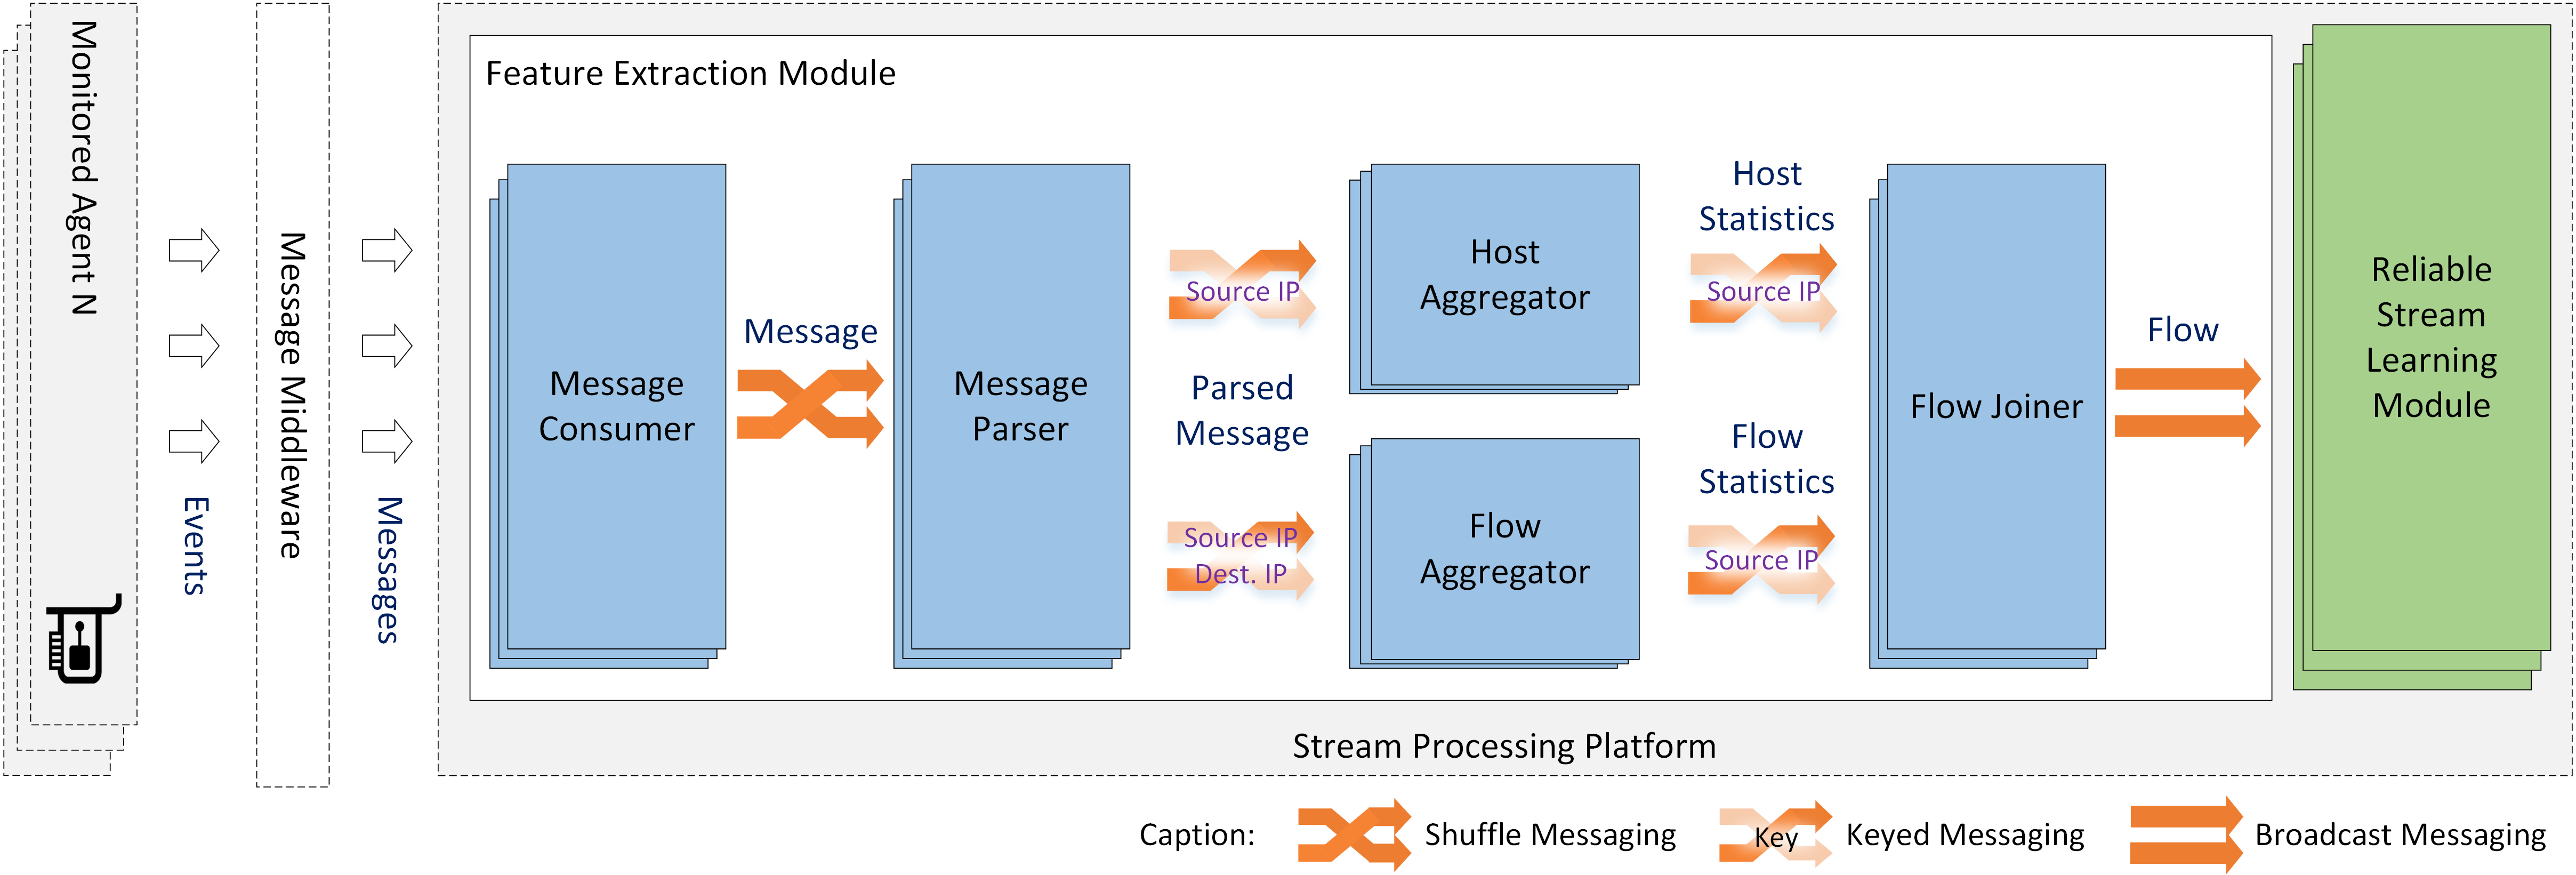
\includegraphics[width=\textwidth]{figuras/bigflow-fig2-feature_extraction_module.png}
\caption{Módulo de extração de atributos da ferramenta BigFlow \cite{Viegas2019}.}
\label{fig:bigflow-pcap}
\end{figure}

\begin{figure}[!ht]
\centering
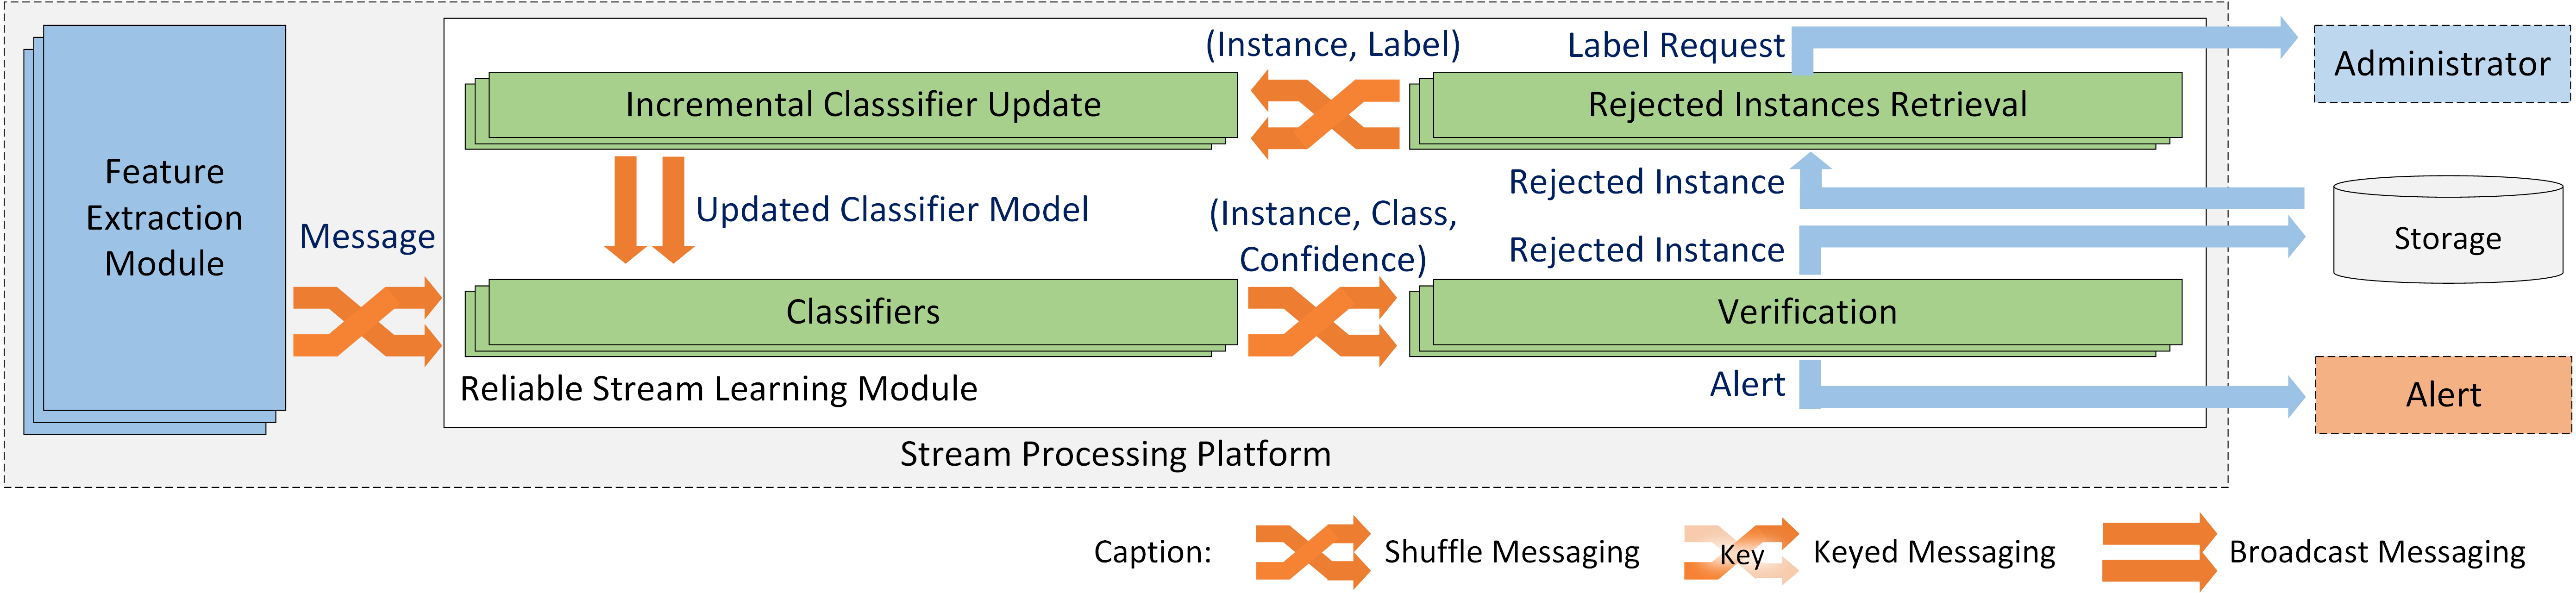
\includegraphics[width=\textwidth]{figuras/bigflow-fig4-reliable_learning_module.png}
\caption{Módulo de aprendizado confiável da ferramenta BigFlow \cite{Viegas2019}.}
\label{fig:bigflow-ml}
\end{figure}

% BigFlow destaca em sua secção 2 (backgroud) o processamento de streams [18, 19],
% a preferencia de NIDS por anomalia em contraste aos NIDS por assinatura [30, 31, 32],
% a variabilidade e evolução dos padrões de tráfego em redes de propósito geral [9, 11, 20],
% a necessidade de atualização regular do modelo classificador [8, 9, 10, 20] e
% o tratamento de eventos onde a confiança resultante da classificação é baixa [9, 12, 13].

% [22] MAWI Working Group Traffic Archive, http://mawi.wide.ad.jp/mawi/samplepoint-F/.
% [24] H. He, E.A. Garcia, Learning from imbalanced data, IEEE Trans. Knowl. Data Eng.
% 21 (2009) 1263–1284. doi:10.1109/TKDE.2008.239.

\citeonline{Viegas2019} destaca que \datasets adequados para NIDS são
poucos devido o conjunto de qualidades que os mesmos devem atender como
realismo, validade, etiquetamento, grande variabilidade e reprodutividade
(disponibilidade pública).

Para avaliar o desempenho de NIDS o \dataset MAWIFlow é proposto por \citeonline{Viegas2019}.
Originário do
\dataset \emph{Packet traces from WIDE backbone, samplepoint-F} composto por
seções de captura de pacotes diárias de 15 minutos de um link de $1
\mathrm{Gbps}$ entre Japão e EUA, com início em 2006 continuamente até hoje,
anonimizados e etiquetados por MAWILab \cite{mawiSamplepointF,Fontugne2010}.
Desse \dataset original, o \dataset MAWIFlow utiliza apenas os eventos de 2016
dos quais 158 atributos são extraídos resultando em 7.9 TB de captura de pacotes.
Além disso, os dados são estratificados para redução de seu tamanho a um
centésimo mantendo as proporções de etiquetas (Ataque e Normal) facilitando o
compartilhamento e avaliação de NIDS além de atender às qualidades anteriormente
mencionadas.

% classifiers that are usually employed for intrusion detection: decision tree
% (DT) [42], random forest (RF) [43], gradient boosting (GB) [44], and an ensemble
% [45] classifier composed from DT, RF, and GB that decides based on majority
% voting across each classifier’s decisions.

Com o \dataset MAWIFlow reduzido a 62 atributos foram avaliados quatro
classificadores da literatura em dois modos de operação.
% quanto aoseus dados de treinamento (ambos contendo uma semana de captura).
O primeiro modo de operação usa somente a primeira semana do ano como conjunto
de treinamento e as demais como conjunto teste.
O segundo modo usando o conjunto da semana anterior como treinamento e o
conjunto da semana seguinte como teste.
Comparando os resultados entre os modos de operação, os autores demonstram que a qualidade da
classificação reduz com o tempo quando não há atualização frequente do modelo
classificador.

Com base na avaliação dos classificadores da literatura, para a ferramenta
BigFlow é proposta a utilização de 4 algoritmos de classificação com capacidade
de atualização, todos algoritmos são variações de árvore de decisão
\emph{Hoeffding} \cite{Viegas2019,Domingos2000}.
A avaliação da ferramenta foi executada de maneira semelhante à avaliação
dos algoritmos da literatura, onde o conjunto de dados da primeira semana foi
usado para treinamento e o conjunto de dados do restante do ano como conjunto
de teste.
Além do conjunto de treinamento, o modelo é atualizado semanalmente com base nas
instâncias rejeitadas pelo submódulo de verificação, como ilustrado na
\reffig{bigflow-ml}.

% four stream learning classifiers were evaluated:
% Hoeffding Tree [51], OzaBoosting [54], Leveraging Bag [55],
% and an Ensemble of the prior three classifiers that performs
% majority voting on the individual outcomes.

\newcommand{\kafka}{\emph{Apache Kafka}\xspace}
\newcommand{\flink}{\emph{Apache Flink}\xspace}

Quanto a distribuição do processamento, ilustrada na \reffig{bigflow-arch},
a ferramenta BigFlow faz uso das plataformas \flink e \kafka.
Em especial, destaca-se o uso do serviço gerenciador de trabalhos (\emph{Job
Manager}) e as múltiplas instâncias do serviço gerenciador de tarefas
(\emph{Task Manager}).

\begin{figure}[ht]
    \centering
    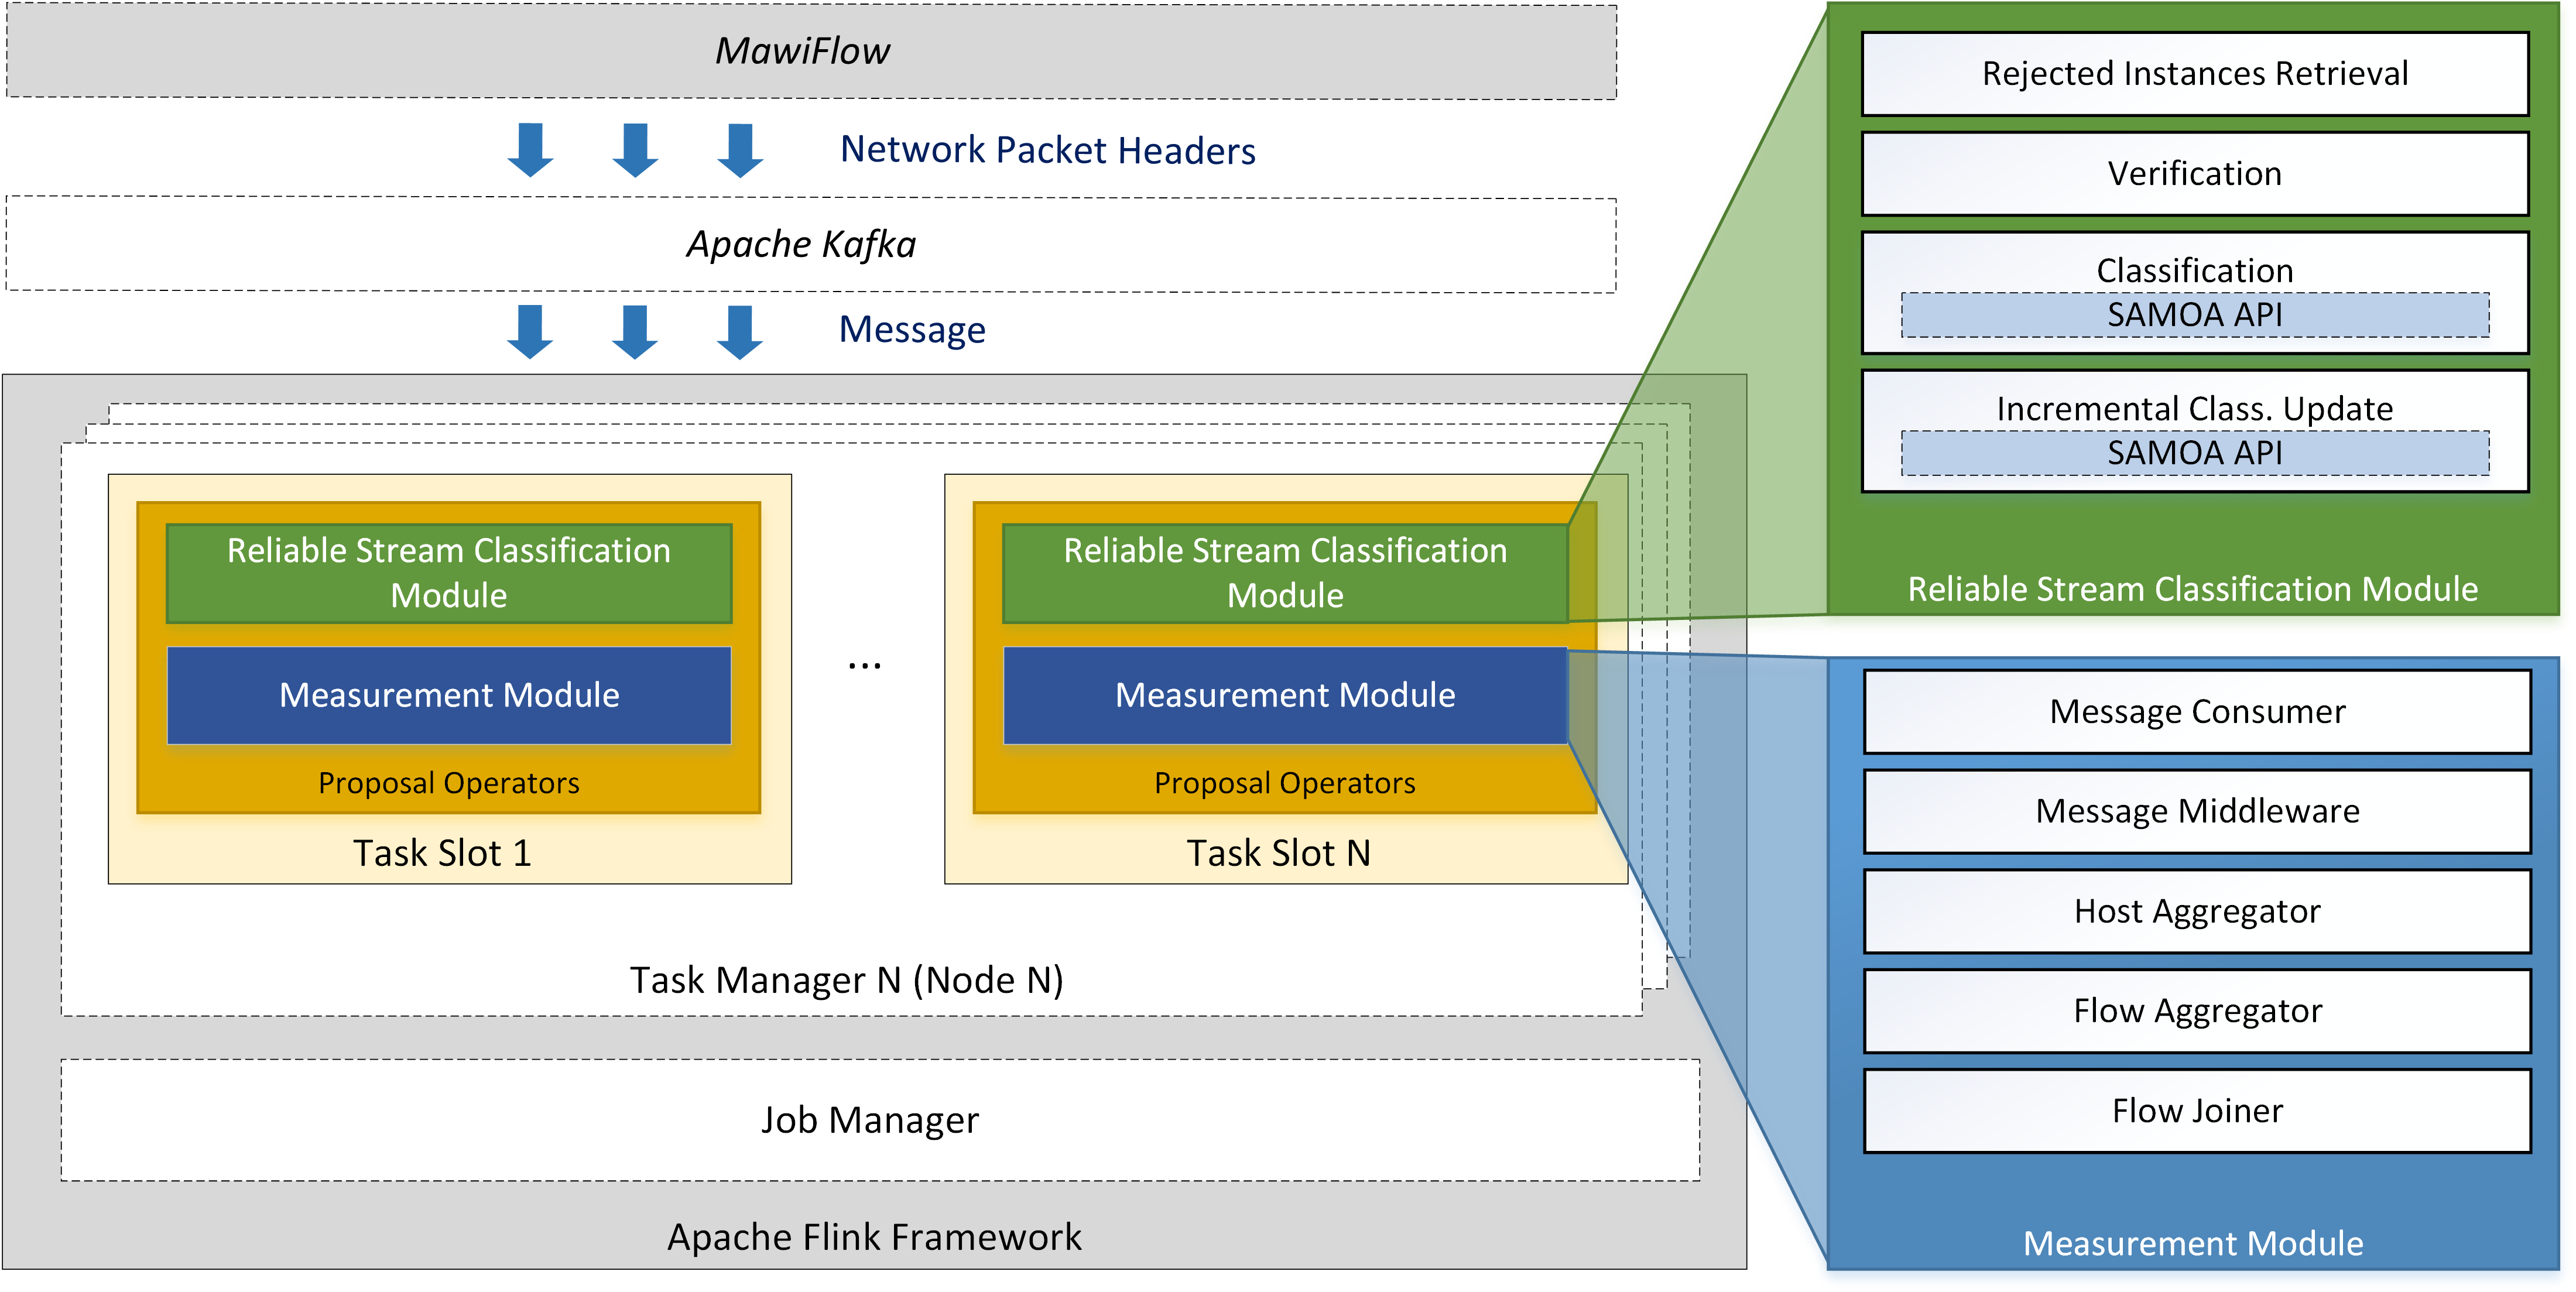
\includegraphics[width=\textwidth]{figuras/bigflow-fig5-bigflow_arch.png}
    \caption{Visão geral da arquitetura e distribuição da ferramenta BigFlow \cite{Viegas2019}.}
    \label{fig:bigflow-arch}
\end{figure}

Em conclusão, a ferramenta BigFlow demonstra a capacidade de classificação e
detecção de anomalias em fluxos de dados de alta velocidade no contexto de
detecção de intrusão.
No entanto, a atualização semanal e, mais importante, dependendo de avaliação de um
especialista, não é ideal para detecção de novidades e respectiva ação sobre a
descoberta de novos padrões.

% Outras propostas tratam do caso de grandes volumes e velocidades, como ́e o caso
% de Viegaset al. (2019) que apresenta oBigFlowno intuito de detectar intrus ̃ao
% em redes10 GigabitEthernet, que ́e um volume consider ́avel atualmente imposs
% ́ıvel de ser processado em um ́unicon ́ucleo de processador (single-threaded).
% Essa implementac ̧ ̃ao ́e feita sobre uma plataformadistribu ́ıda processadora
% de fluxos (Apache Flink) executada em um cluster com at ́e 10 n ́os detrabalho,
% cada um com 4 n ́ucleos de processamento totalizando 40 n ́ucleos para atingir
% taxas deat ́e 10,72Gb ps.

\subsection{Ferramenta CATRACA}

O trabalho \citeonline{Lopez2018} aborda a detecção de ameaças a redes de
computadores em tempo real e para atingir esse objetivo, propôs a ferramenta
CATRACA\footnote{
    A ferramenta e sua documentação estão disponíveis em \url{http://gta.ufrj.br/catraca}
    e \url{https://github.com/tinchoa/catraca}.
}.
A ferramenta CATRACA é composta de três camadas: captura, processamento e
visualização, ilustradas na Figura \ref{fig:catraca}.

\begin{figure}[ht]
\centering
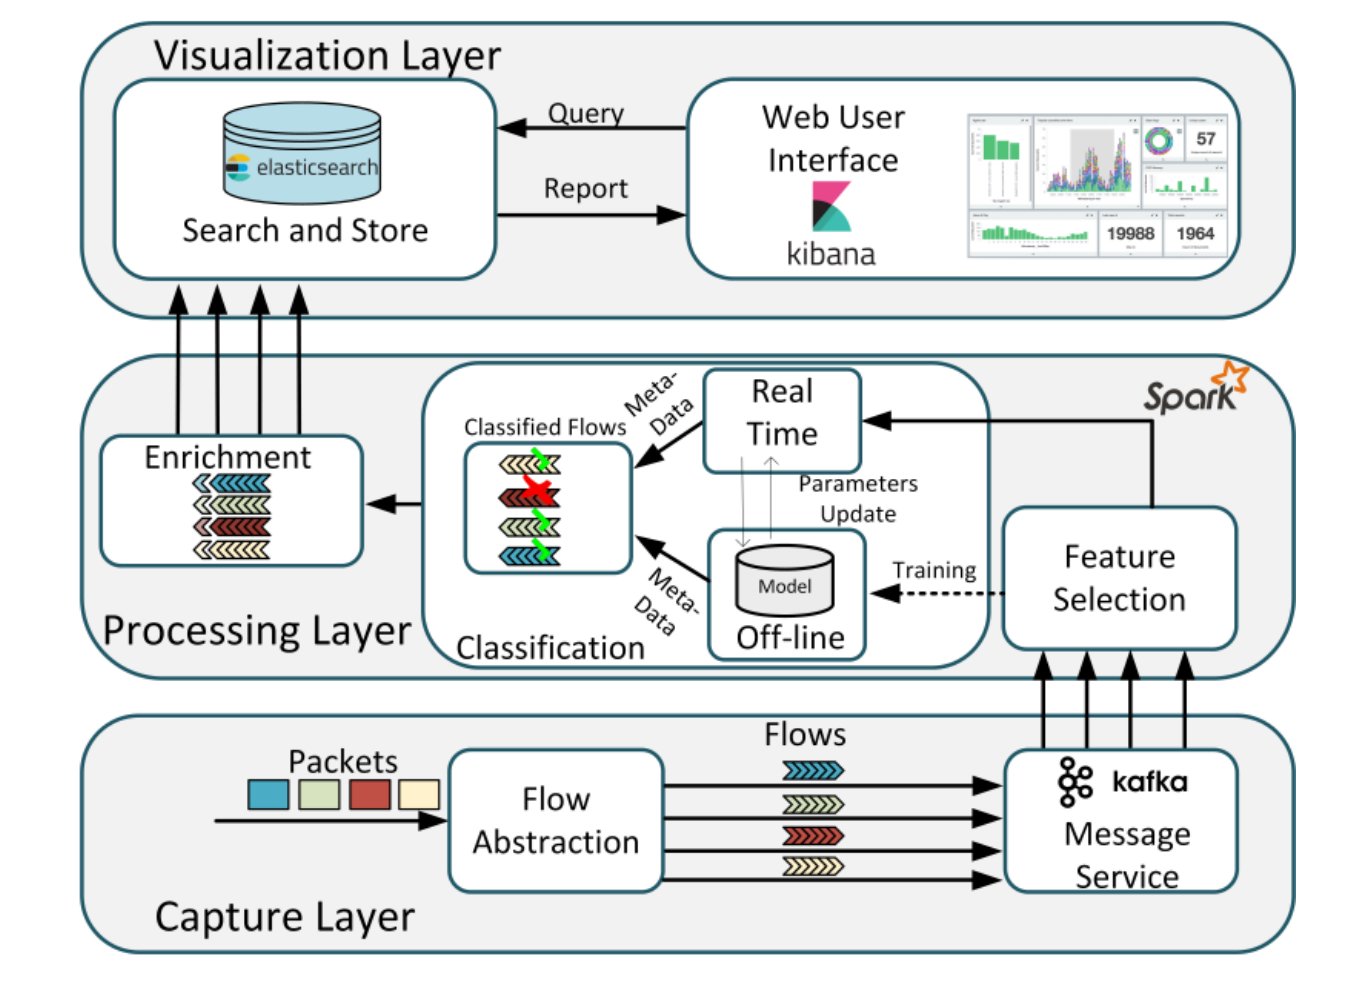
\includegraphics[width=0.8\textwidth]{figuras/catraca-arch.png}
\caption{Arquitetura em camadas da ferramenta CATRACA \cite{Lopez2018}.}
\label{fig:catraca}
\end{figure}

% \nota{deu pra entender,mas coloca ou vírgula, ou divide as frases: baseada na
% biblioteca flowbag. Essa biblioteca é embalada ou a funcao em python esta
% embalada em um funcao virtual de rede?}

Na camada de captura, pacotes são capturados da rede e transformadas em fluxos
por uma aplicação \emph{Python} utilizando a biblioteca \emph{flowtbag}\footnote{
    Disponível em \url{https://github.com/danielarndt/flowtbag} e
    \url{https://dan.arndt.ca/projects/netmate-flowcalc/}.
}
e os fluxos são enviados para um tópico de um sistema de fila de mensagens
(\emph{Apache Kafka}) hospedada em nuvem.
Essa aplicação \emph{Python} é distribuída como uma função virtual de rede
(\emph{Network Function Virtualization}) executada em dispositivos de rede
virtuais.

% estabelecendo um ambiente de computação em névoa.
A camada de processamento consome o tópico de mensagens que contém os fluxos
da camada de captura e extrai características dos fluxos, detecta e classifica ameaças,
enriquece o resultado (com localização geográfica por exemplo) e envia para a
próxima camada na arquitetura por meio de um banco de dados (SGBD).
A última camada da ferramenta fornece uma interface gráfica que apresentada a
visualização dos fluxos processados bem como os conhecimentos extraídos e
armazenados no banco de dados (SGBD).
Ambas camadas de processamento e visualização são executadas em ambiente de
computação em nuvem (\cloud).

Para o desenvolvimento da ferramenta CATRACA, \citeonline{Lopez2018} avaliou e
comparou as plataformas de processamento de fluxo de dados em tempo real
disponíveis (\emph{Apache Storm}, \emph{Apache Flink}, \emph{Apache Spark Streaming}).
A avaliação extraiu a velocidade máxima, em mensagens por minuto,
de cada plataforma variando a configuração de paralelismo
em dois programas, ambos consumiam de um tópico de um sistema de fila
de mensagens (\emph{Apache Kafka}) e produziam para outro tópico.
O primeiro programa consiste de um detector de ameças composto por
uma rede neural classificadora escrito em \emph{Java} e é testado
com o conjunto de dados sintético UFRJ/GTA \cite{Lopez2018}.
O segundo programa conta quantas repetições de uma palavra existem em um
fluxo de dados, exemplo muito comum em tutoriais de plataformas desse gênero,
e é avaliado com um conjunto de \emph{Tweets}.

% Nesta avaliação, \emph{Apache Storm} foi capaz de processar até 15 milhões de
% mensagens por minuto
% 
% We described and compared the three-major open source distributed stream
% processing systems: Apache Storm, Apache Flink, and Apache Spark Streaming. We
% performed throughput analysis, allocating more processing cores to achieve
% higher processing rates, Apache Stormwas able to process up to 15 million
% samples per minute. Moreover, we performed fault tolerance test to compare these
% three most popular open-source Distribute Stream Processors (DSP). In this case,
% we showed that Spark streaming, using micro-batch processing model, can recover
% the failure without losing any messages. Spark Streaming stores the full
% processing state of the micro-batches and distributes the interrupted processing
% homogeneously among other worker nodes.

% A comparação envolveu:
% \begin{enumerate}
%     \item Apache Storm versão 0.9.4 de 2015-03-18 (atualmente na versão 2.1.0,
%     publicada em 2019-10-25);
%     \item Apache Flink versão 0.10.2 de 2016-02-03 (atualmente na versão 1.10.0,
%     publicada em 2020-02-11);
%     \item Apache Spark Streams versão 1.6.1 de 2016-02-27 (atualmente na versão
%     2.4.5, publicada em 2020-02-02);
% \end{enumerate}
% Além das plataformas comparadas é importante mencionar a presença em todos os
% testes do Apache Kafka na versão 0.8.2.1 de 2015-02-26 (atualmente na versão
% 2.4.0 de 2019-12-13).
% A estratégia de avaliação continha um 
% Os resultados apresentados por essa avaliação mostraram que Apache Storm 

Para o modelo de classificação, a ferramenta CATRACA utiliza o método árvore de
decisão, escolhido pelo rápido treinamento e alta precisão e acurácia\footnote{
    A precisão e acurácia do método árvore de decisão pode estar associado
    a independência entre as características (\emph{features}) de cada exemplo
    típicos de conjuntos derivados de pacotes de rede.
}.
O modelo é criado na fase \emph{Offline} e utilizado na classificação binária
(normal e ameaça) da fase \emph{Online}, sendo recalculado quando uma ameaça
é encontrada.

Pra avaliação da ferramenta CATRACA dois conjuntos de dados são utilizados.
O primeiro conjunto, UFRJ/GTA, é sintético criado por uma simulação de rede de
computadores com $214200$ fluxos de rede totalizando $95 \mathrm{GB}$ de pacotes capturados,
é composto de 24 atributos e 16 classes.
O outro conjunto, referido como NetOp, foi coletado de um operador de rede que
atende 373 residências na cidade do Rio de Janeiro em 2017.
O conjunto NetOp é formado por 5 TB de pacotes capturados e etiquetados por um
detector de intrusão comercial.

Também para a avaliação da ferramenta CATRACA, utilizou-se as métricas de qualidade
de classificação acurácia, precisão, sensibilidade e F1M com intervalo de
confiança de 95\%.
As métricas de qualidade, dependendo do tamanho do conjunto, foram extraídas por
métodos de avaliação amplamente utilizados para avaliar modelos de aprendizado
de máquina (\emph{machine learning}) como validação cruzada com proporção
70\% do conjunto base para treinamento e 30\% para teste.
Para as métricas de escalabilidade utiliza latência e fator de aceleração
\emph{speedup factor} (latência observada com paralelismo 1 dividida pela
latência observada com paralelismo variável).

Em conclusão, a ferramenta CATRACA apresenta uma arquitetura dividida em camadas
alocadas em ambientes de névoa (\fog) e nuvem (\cloud), essa ferramenta é
avaliada com métricas e dois conjuntos de dados relevantes.
No entanto, o algoritmo de detecção de anomalias desenvolvido para a ferramenta
consiste de um modelo de classificação pelo método árvore de decisão e
a atualização do modelo durante a fase \emph{Online} depende de todos os exemplos do
último intervalo de atualização.
Esse tipo de algoritmo de detecção de anomalias não é capaz de lidar
adequadamente com as características de fluxos contínuos de dados como os
descritos na \refsec{nd} (\drift, \evolution, limitado a ler o conjunto somente
uma vez) que são atendidos por algoritmos de detecção de novidade.

% A monitoring and threat detection system using stream processing as a virtual 
% function for Big Data

% A detecção tardia de ameaças de segurança causa um significante aumento no
% risco de danos irreparáveis, impossibilitando qualquer tentativa de defesa.
% Como consequência, a detecção rápida de ameaças em tempo real é essencial
% para a ad- ministração de segurança. Além disso, A tecnologia de
% virtualização de funções de rede (Network Function Virtualization - NFV)
% oferece novas oportunidades para soluções de segurança eficazes e de baixo
% custo. Propomos um sistema de detecção de ameaças rápido e eficiente,
% baseado em algoritmos de processamento de fluxo e de aprendizado de máquina. As
% principais contribuições deste trabalho são: 
% i) um novo sistema de monitoramento e detecção de ameaças baseado no processamento de fluxo; 
% ii) dois conjuntos de dados, o primeiro é um conjunto de dados sintético de
% segurança contendo tráfego suspeito e malicioso, e o segundo corresponde a uma
% semana de tráfego real de um operador de telecomunicações no Rio de Janeiro,
% Brasil; 
% iii) um algoritmo de pré-processamento de dados composto por um algoritmo
% de normalização e um algoritmo para seleção rápida de
% características com base na correlação entre variáveis;
% iv) uma função de
% rede virtualizada em uma plataforma de código aberto para fornecer um serviço
% de detecção de ameaças em tempo real;
% v) posicionamento quase perfeito de
% sensores através de uma heurística proposta para posicionamento estratégico
% de sensores na infraestrutura de rede, com um número mínimo de sensores; e,
% finalmente, 
% vi) um algoritmo guloso que aloca sob demanda uma sequência de 
% funções de rede virtual.

\section{Arquitetura \idsiot}\label{sec:cassales}

A arquitetura \idsiot, proposta por \citeonline{Cassales2019a}, tem por objetivo
monitorar uma rede local com dispositivos \iot e detectar tentativas de intrusão
e até possível subversão destes dispositivos.
O principal destaque da arquitetura é a distribuição de tarefas do sistema de
detecção de intrusão entre nós na rede de borda (\fog) e nós em nuvem pública
(\cloud).
O objetivo dessa distribuição é a redução de latência que torna inviável a
hospedagem de um sistema detector de intrusão somente em ambiente \cloud e
também possibilitar a análise de grandes volumes de dados por algoritmos de
maior complexidade que são de custo computacional proibitivo para nós de borda.
A \reffig{ids-iot-phy} ilustra a estrutura física da arquitetura \idsiot,
destacando os dispositivos \iot, dispositivos de borda e nuvem pública.

\begin{figure}[ht]
\centering
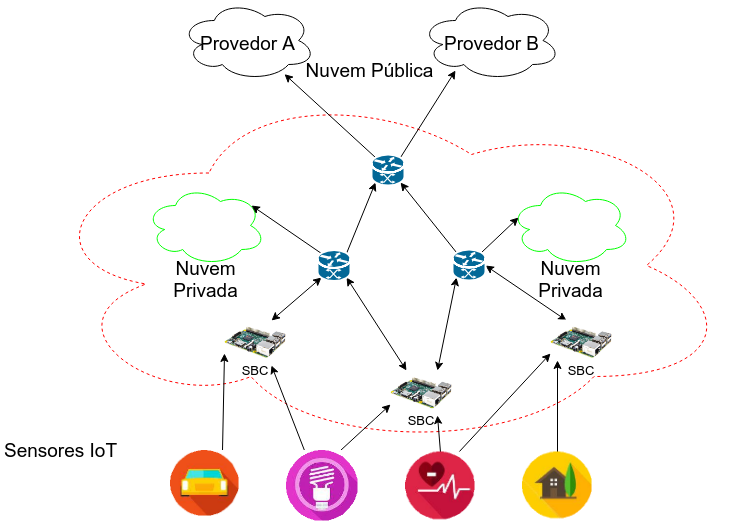
\includegraphics[width=0.8\textwidth]{figuras/idsa-iot-quali-000.png}
\caption{Estrutura Física da Arquitetura \idsiot.
Produzida e traduzida por \citeonline{Cassales2019a}.}
\label{fig:ids-iot-phy}
\end{figure}

A arquitetura proposta é avaliada com três algoritmos de detecção de novidade:
ECSMiner \cite{Masud2010ECSMiner}, AnyNovel \cite{Abdallah2016anynovel} e MINAS
\cite{Faria2016minas}.
A avaliação foi feita com o \dataset \emph{Kyoto 2006+}, composto de
dados coletados de 348 \emph{Honeypots} (máquinas isoladas com diversos
softwares com vulnerabilidades conhecidas expostas à Internet com propósito de
atrair ataques) de 2006 até dezembro 2015.
Esse \dataset tem as características desejáveis de um conjunto para detectção de
novidades como: realismo, validade, etiquetas previamente definidas, alta
variabilidade, reprodutibilidade e disponibilidade pública.
O \dataset \emph{Kyoto 2006+} contém 24 atributos, 3 etiquetas atribuídas por
detectores de intrusão comerciais e uma etiqueta
distinguindo o tráfego entre normal, ataque conhecido e ataque desconhecido.

A avaliação da arquitetura foi realizada utilizando as métricas de qualidade
Fnew, Mnew e erro.
A métrica Fnew (ou Falso Positivo) é a fração dos exemplos de uma classe normal
classificados com etiqueta novidade ou etiqueta extensão.
A métrica Mnew (ou Falso Negativo) é a fração dos exemplos de uma classe novidade
classificados com etiqueta normal.
A métrica erro é a soma dos valores falso positivo e falso negativo dividida
pelo número de exemplos classificados.
Além das métricas de qualidade de classificação tradicionais, também foi medida
a quantidade de requisições de classificação por especialista.

Outra avaliação dos algoritmos foi a extração de métricas de uso de recursos
computacionais e tempo total de processamento em dispositivos limitados.
Essa avalição envolveu dois computadores, um computador pessoal com recursos
convecionais produzia exemplos e adicionava como mensagens em um tópico no
sistema de fila de mensagens \kafka, já o outro computador com recursos
limitados consumia as mensagens do tópico e classificava os exemplos.

Ambas as avaliações demonstraram o equilíbrio entre qualidade de classificação e
velocidade ou uso de recursos.
O algoritmo ECSMiner mostrou melhor qualidade de classificação, porém com
velocidade inferior e maior consumo de recursos comparado aos outros algoritmos.
Já o algoritmo MINAS, apesar de maiores valores na métrica erro, mostrou-se
adequado para dispositivos limitados com baixo consumo de recursos
computacionais e manteve constante e baixa métrica Fnew.
O algoritmo AnyNovel não apresentou consistência nos resultados e o consumo
de recursos computacionais (memória) foi elevado.

% MINAS technique presented high error rates. However, the
% small and constant Fnew coupled with the smallest execution
% time and memory consumption, indicates MINAS is suitable
% for IoT scenarios.

Com as avaliações realizadas, a arquitetura \idsiot opta por distribuir as
tarefas de mineração dos fluxos para detecção de intrusão em serviços e aloca os
serviços em diferentes camadas físicas conforme ilustrado na \reffig{ids-iot}.

\begin{figure}[hbt]
\centering
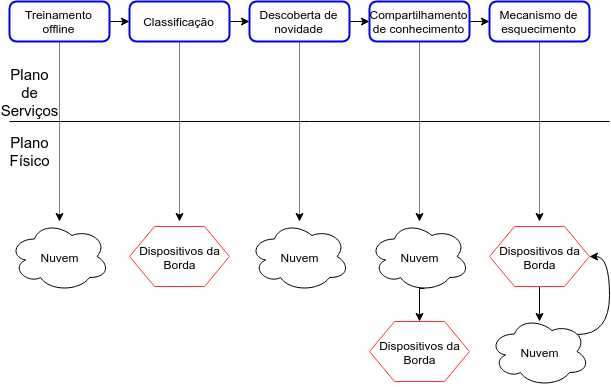
\includegraphics[width=0.8\textwidth]{figuras/idsa-iot-quali-004.png}
\caption{Distribuição de Serviços da Arquitetura \idsiot.
Produzida e traduzida por \citeonline{Cassales2019a}.}
\label{fig:ids-iot}
\end{figure}

A distribuição das tarefas em serviços proposta abre oportunidades para a
discussão de diferentes métodos de distribuição dessas tarefas em diferentes
ambientes computacionais.
Contudo, o algoritmo MINAS ainda não foi implementado e avaliado com
paralelismo, multi-processamento ou distribuição computacional, que são
necessários para tratar fluxos de dados com grandes volumes e velocidades.

% \nota{Também discutir a classificação dos fluxos por endpoint
% exarcerbando assim a distinção na fog com o efeito de particionamento dos dados.
% Ou seja, um nó só vê e classifica os próprios dados.}

% \section{Conjuntos de Dados e Referência de Desempenho para Detecção de Anomalia}

% The Numenta Anomaly Benchmark
% - Airline, approximately 116 million flight arrival and departure records
%   (cleaned and sorted) compiled by E. Ikonomovska. Reference: Data Expo 2009
%   Competition [1]. Access
% - Chess.com (online games) and Luxembourg (social survey) datasets compiled by
%   I. Zliobaite. Access
% - ECUE spam 2 datasets each consisting of more than 10,000 emails collected over
%   a period of approximately 2 years by an individual. Access from S.J.Delany
%   webpage
% - Elec2, electricity demand, 2 classes, 45,312 instances. Reference: M. Harries,
%   Splice-2 comparative evaluation: Electricity pricing, Technical report, The
%   University of South Wales, 1999. Access from J.Gama webpage. Comment on
%   applicability.
% - PAKDD'09 competition data represents the credit evaluation task. It is
%   collected over a five-year period. Unfortunately, the true labels are released
%   only for the first part of the data. Access
% - Sensor stream and Power supply stream datasets are available from X. Zhu's
%   Stream Data Mining Repository. Access
% - SMEAR is a benchmark data stream with a lot of missing values. Environment
%   observation data over 7 years. Predict cloudiness. Access
% - Text mining, a collection of text mining datasets with concept drift,
%   maintained by I. Katakis. Access
% - Gas Sensor Array Drift Dataset, a collection of 13,910 measurements from 16
%   chemical sensors utilized for drift compensation in a discrimination task of 6
%   gases at various levels of concentrations. Access

\newcommand{\stream}{\emph{data stream}\xspace}
\newcommand{\streams}{\emph{data streams}\xspace}
\newcommand{\streamMining}{\emph{data stream mining}\xspace}

\section{Conclusão}\label{sec:conclusao-relacionados}

% \nota{coloca uma secao de SINTESE dos trabalhos relacionados ou sintese do capitulo}

Em conclusão, os trabalhos discutidos nesse Capítulo tem temas complementares em
áreas distintas.
A área de aprendizado de máquina, com o tema detecção de novidades em fluxos de
dados, preocupa-se em fornecer melhores previsões através de algoritmos
classificadores que atendam as características de cada problema.
A área de computação distribuída, aborda os temas de processamento distribuído
de fluxos contínuos em ambientes de computação em nuvem e em névoa, fornecendo
métodos para processar grandes volume de dados com mínima latência.

Apesar de já existirem propostas que estabelecem o estado da arte separadamente
em cada um dos temas, falta ainda uma abordagem que estabeleça uma união entre o
estado da arte em algoritmos de detecção de novidade e o estado da arte em
processamento distribuído de fluxos de dados, em especial para o ambiente de
computação em névoa focado em fluxos de dados relacionados a dispositivos \iot.
